
\documentclass[11pt]{exam} % https://www.ctan.org/pkg/exam?lang=en

\usepackage[lmargin=1.in,rmargin=1.in,tmargin=1.in,bmargin=1in]{geometry}
\usepackage{setspace}
\usepackage[pdftex]{graphicx}
\usepackage{titling}
\usepackage[
	pdfauthor={Brian Weinstein},
	pdftitle={Homework 3},
	bookmarks=true,
	colorlinks=true,
	linkcolor=blue,
	urlcolor=blue,
	citecolor=blue,
	pdftex,
	linktocpage=true
	]{hyperref}
\usepackage[textsize=tiny]{todonotes}
\usepackage{float}
\setlength\parindent{0pt}
\usepackage{lipsum}


\qformat{\textbf{Problem \thequestion: \thequestiontitle}\quad \hfill}


\pagestyle{headandfoot}
\runningheadrule
\firstpageheader{}{}{}
\runningheader{\thetitle}{\theauthor}{\thedate}
\firstpagefooter{}{\thepage}{}
\runningfooter{}{\thepage}{}


\usepackage{xcolor}
\usepackage{adjustbox}
\usepackage{verbatim}
\definecolor{shadecolor}{rgb}{.9, .9, .9}

\newenvironment{code}%
   {\par\noindent\adjustbox{margin=1ex,bgcolor=shadecolor,margin=0ex \medskipamount}\bgroup\minipage\linewidth\verbatim}%
   {\endverbatim\endminipage\egroup}

\newenvironment{codeSmall}%
   {\par\noindent\adjustbox{margin=1ex,bgcolor=shadecolor,margin=0ex \medskipamount}\bgroup\minipage\linewidth\verbatim\footnotesize}%
   {\endverbatim\endminipage\egroup}





\begin{document}


\title{STAT S4240 002, Homework 3}
\author{Brian Weinstein (bmw2148)}
\date{July 30, 2015}
\maketitle



\begin{questions}



\titledquestion{Naive Bayes Text Classification: Data Preparation}

See \texttt{hw03\_q1.R} for code.

\begin{parts}

\part Text pre-processing
\begin{codeSmall}
# load functions from hw03.R
source("hw03.R")

# preprocess text
preprocess.directory("datasets/FederalistPapers/fp_hamilton_train")
preprocess.directory("datasets/FederalistPapers/fp_hamilton_test")
preprocess.directory("datasets/FederalistPapers/fp_madison_train")
preprocess.directory("datasets/FederalistPapers/fp_madison_test")
\end{codeSmall}

\part Loading the cleaned data
\begin{codeSmall}
hamilton.train <- read.directory("datasets/FederalistPapers/fp_hamilton_train_clean")
hamilton.test <- read.directory("datasets/FederalistPapers/fp_hamilton_test_clean")
madison.train <- read.directory("datasets/FederalistPapers/fp_madison_train_clean")
madison.test <- read.directory("datasets/FederalistPapers/fp_madison_test_clean")
\end{codeSmall}


\part Create a dictionary from all of the documents
\begin{codeSmall}
dictionary <- make.sorted.dictionary.df(c(hamilton.train, hamilton.test,
                                          madison.train, madison.test))
\end{codeSmall}




\part Creating document-term-matrices for each of the datasets
\begin{codeSmall}
dtm.hamilton.train <- make.document.term.matrix(infiles=hamilton.train,
                                                dictionary=dictionary)
dtm.hamilton.test <- make.document.term.matrix(infiles=hamilton.test,
                                               dictionary=dictionary)
dtm.madison.train <- make.document.term.matrix(infiles=madison.train,
                                               dictionary=dictionary)
dtm.madison.test <- make.document.term.matrix(infiles=madison.test,
                                              dictionary=dictionary)
\end{codeSmall}







\part Compute the log probabilities for the dictionary in each of the document datasets
\begin{codeSmall}
mu=1/nrow(dictionary)

logp.hamilton.train <- make.log.pvec(dtm.hamilton.train, mu)
logp.hamilton.test <- make.log.pvec(dtm.hamilton.test, mu)
logp.madison.train <- make.log.pvec(dtm.madison.train, mu)
logp.madison.test <- make.log.pvec(dtm.madison.test, mu)
\end{codeSmall}

\end{parts}



\titledquestion{Naive Bayes Function}

We first estimate the log priors based on the log of the proportion of training documents attributed to each author.

$$p(\textrm{author}=\texttt{author})=\log\left(\frac{\textrm{\# of training documents attributed to }\texttt{author}}{\textrm{total \# of training documents}}\right)$$

Then, using (1) the log probabilities for the dictionary in a Hamilton-authored document and (2) the log probabilities for the dictionary in a Madison-authored document (as computed in \textbf{Problem 1}), we can input a new document-term-matrix and classify each document as belonging to one of the authors.

\begin{code}
naive.bayes <- function(logp.hamilton.train, logp.madison.train,
                        log.prior.hamilton, log.prior.madison, dtm.test){
  # Performs naive bayes classification
  # Inputs:  logp.hamilton.train  :   vector of log probabilities of words
  #                                     occurring in the hamilton training data
  #          logp.madison.train   :   vector of log probabilities of words
  #                                     occurring in the madison training data
  #          log.prior.hamilton   :   the log prior of hamilton documents
  #          log.prior.madison    :   the log prior of madison documents 
  #          dtm.test             :   a document-term-matrix to classify
  # Output:  Classification labels for each document in dtm.test
  
  # calculate the log posterior probabilities
  log.post.hamilton <- log.prior.hamilton + (dtm.test %*% logp.hamilton.train)
  log.post.madison <- log.prior.madison + (dtm.test %*% logp.madison.train)
  
  # compare the log posterior probabilities and assign to the author
  # with highest probability
  prediction <- data.frame(logPostHam=log.post.hamilton,
                           logPostMad=log.post.madison)
  prediction$pred <- (log.post.hamilton >= log.post.madison)
  prediction$pred <- gsub(TRUE, "Hamilton", prediction$pred)
  prediction$pred <- gsub(FALSE, "Madison", prediction$pred)
  
  # return a vector of the predictions
  return(prediction$pred)
  
}
\end{code}

\titledquestion{Assessing Model Performance}

\begin{itemize}
\item \textbf{Accuracy:} 63\% accurate (\% of the test papers that are classified correctly)
\item \textbf{True Positive Rate:} 100\% (Hamilton classified as Hamilton divided by the total amount of testing Hamilton papers)
\item \textbf{True Negative Rate:} 9\% (Madison classified as Madison divided by the total amount of testing Madison papers)
\item \textbf{False Positive Rate:} 91\% (Madison classified as Hamilton divided by the total amount of testing Madison)
\item \textbf{False Negative Rate:} 0\% (Hamilton classified as Madison divided by the total amount of testing Hamilton)
\end{itemize}


\begin{code}
> confusionMatrix(data=predictions$pred,
+                 reference=predictions$trueValue,
+                 dnn=c("Prediction", "True Value"),
+                 positive="Hamilton")
Confusion Matrix and Statistics

          True Value
Prediction Hamilton Madison
  Hamilton       16      10
  Madison         0       1
                                         
               Accuracy : 0.6296         
                 95% CI : (0.4237, 0.806)
    No Information Rate : 0.5926         
    P-Value [Acc > NIR] : 0.427258       
                                         
                  Kappa : 0.106          
 Mcnemar's Test P-Value : 0.004427       
                                         
            Sensitivity : 1.00000        
            Specificity : 0.09091        
         Pos Pred Value : 0.61538        
         Neg Pred Value : 1.00000        
             Prevalence : 0.59259        
         Detection Rate : 0.59259        
   Detection Prevalence : 0.96296        
      Balanced Accuracy : 0.54545        
                                         
       'Positive' Class : Hamilton       
\end{code}




\titledquestion{5-fold Cross Validation}

\begin{parts}

\part \textbf{5-Fold Cross-Validation}\ \ For each value of $\mu \in \left\{ \frac{0.1}{\left|D\right|}, \frac{1}{\left|D\right|}, \frac{10}{\left|D\right|}, \frac{100}{\left|D\right|}\frac{1000}{\left|D\right|} \right\}$, where $\left|D\right|=4875$ is the size of our dictionary; estimations of the the correct classification rate, the false negative rate, and the false positive rate are outlined below. For each of the metrics, the table indicates the value for each of the 25 tests and the graph indicates averages over the 5 tests for each choice of $\mu$.
\smallskip

\textbf{Correct Rate:}
\begin{code}
    fold1 fold2 fold3 fold4 fold5
mu1   0.7   0.7   0.7   0.7   0.7
mu2   0.8   0.7   0.7   0.7   0.7
mu3   0.8   0.7   0.7   0.8   0.8
mu4   0.9   0.7   0.8   0.8   1.0
mu5   1.0   0.8   0.9   0.8   1.0
\end{code}

\begin{figure}[H]
	\centering
	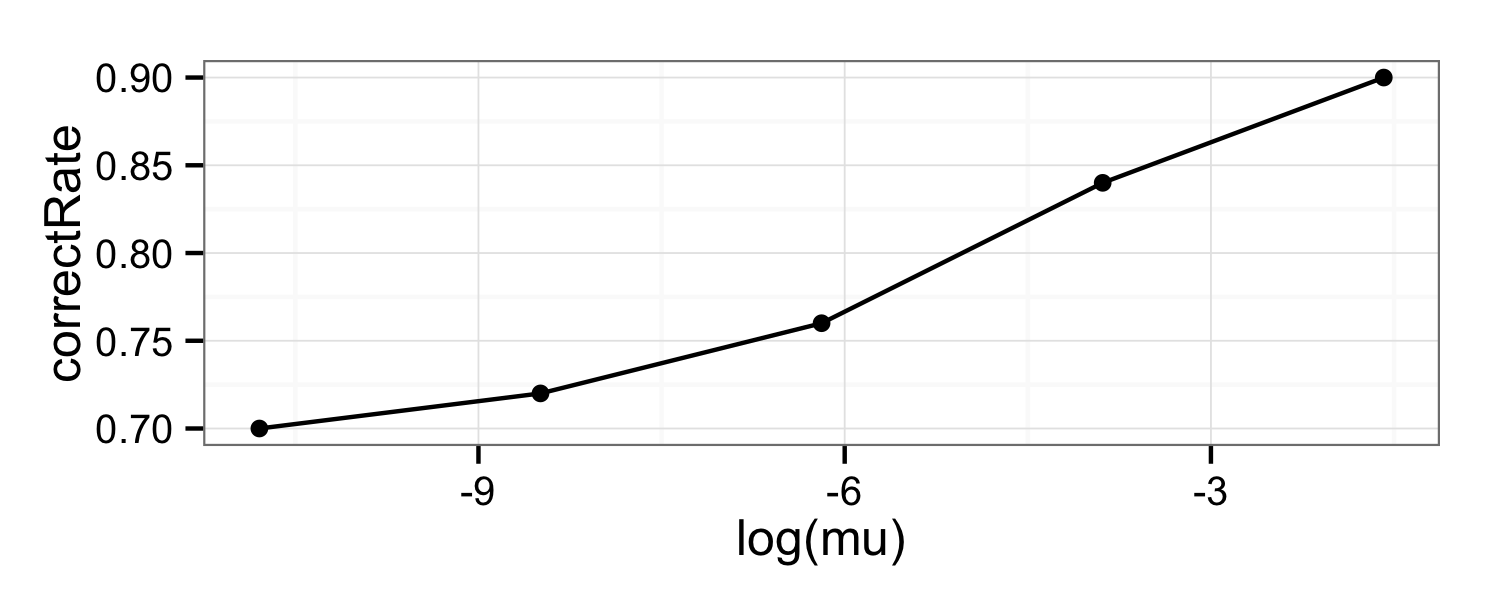
\includegraphics[width=5in]{4a_correctRate.png}
	%\caption{}
	%\label{fig:figName}
\end{figure}

\textbf{False Negative Rate:}
\begin{code}
    fold1 fold2 fold3 fold4 fold5
mu1     0     0     0     0     0
mu2     0     0     0     0     0
mu3     0     0     0     0     0
mu4     0     0     0     0     0
mu5     0     0     0     0     0
\end{code}

\begin{figure}[H]
	\centering
	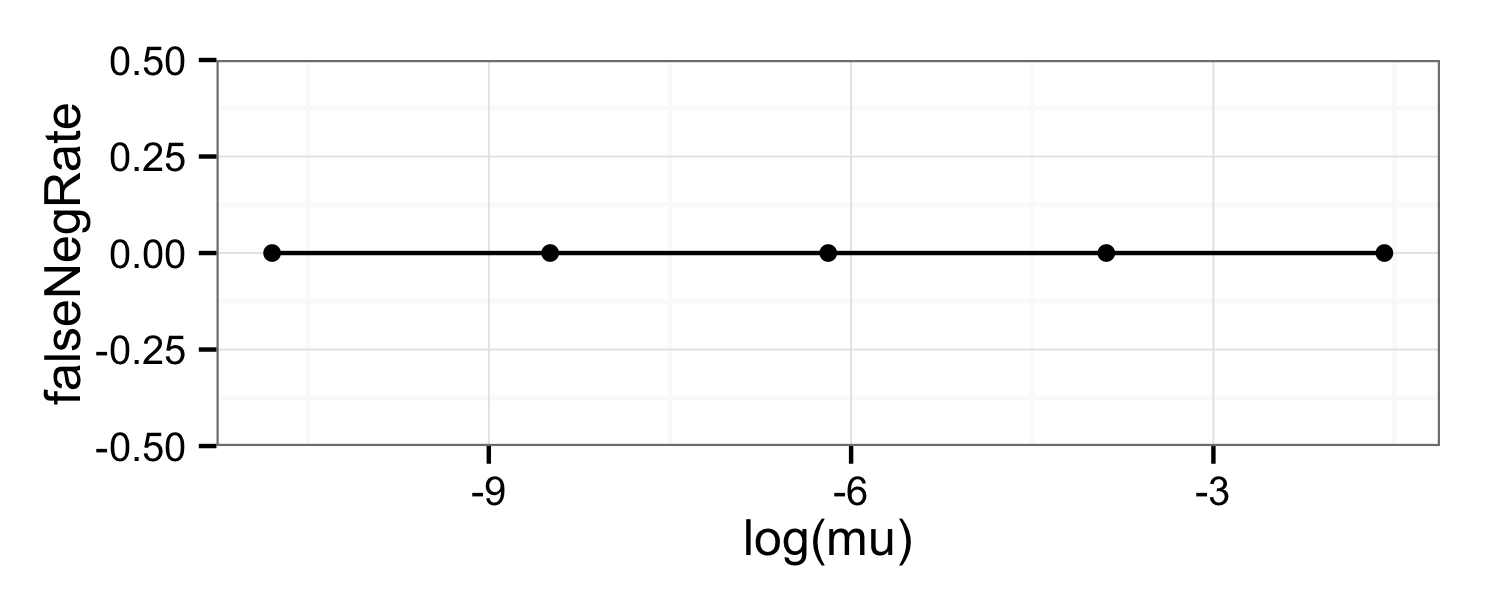
\includegraphics[width=5in]{4a_falseNegRate.png}
	%\caption{}
	%\label{fig:figName}
\end{figure}

\textbf{False Positive Rate:}
\begin{code}
        fold1     fold2     fold3     fold4     fold5
mu1 1.0000000 1.0000000 1.0000000 1.0000000 1.0000000
mu2 0.6666667 1.0000000 1.0000000 1.0000000 1.0000000
mu3 0.6666667 1.0000000 1.0000000 0.6666667 0.6666667
mu4 0.3333333 1.0000000 0.6666667 0.6666667 0.0000000
mu5 0.0000000 0.6666667 0.3333333 0.6666667 0.0000000
\end{code}

\begin{figure}[H]
	\centering
	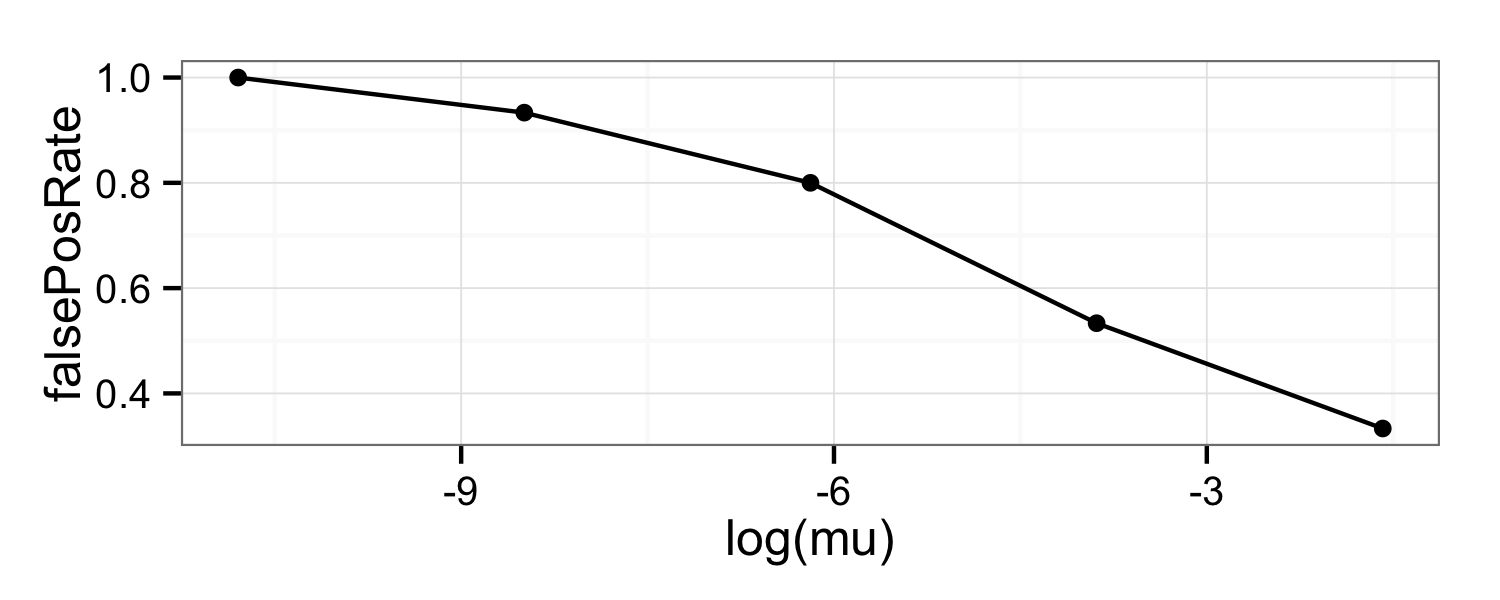
\includegraphics[width=5in]{4a_falsePosRate.png}
	%\caption{}
	%\label{fig:figName}
\end{figure}



\part Based on the values measured on the training set (using 5-fold cross validation), the best value for $\mu$ is \texttt{mu5} $=\frac{1000}{\left|D\right|}\approx0.205$. At this value we maximize the accuracy and minimize the false positive rate, with no increase in the false negative rate.

\part \textbf{Testing Set}\ \ For the same values of $\mu$ used in Part (a), estimations of the the correct classification rate, the false negative rate, and the false positive rate are outlined below.
\smallskip

\textbf{Correct Rate:}
\begin{code}
              mu1       mu2       mu3       mu4       mu5
testSet 0.6296296 0.6296296 0.7037037 0.8518519 0.9259259
\end{code}

\begin{figure}[H]
	\centering
	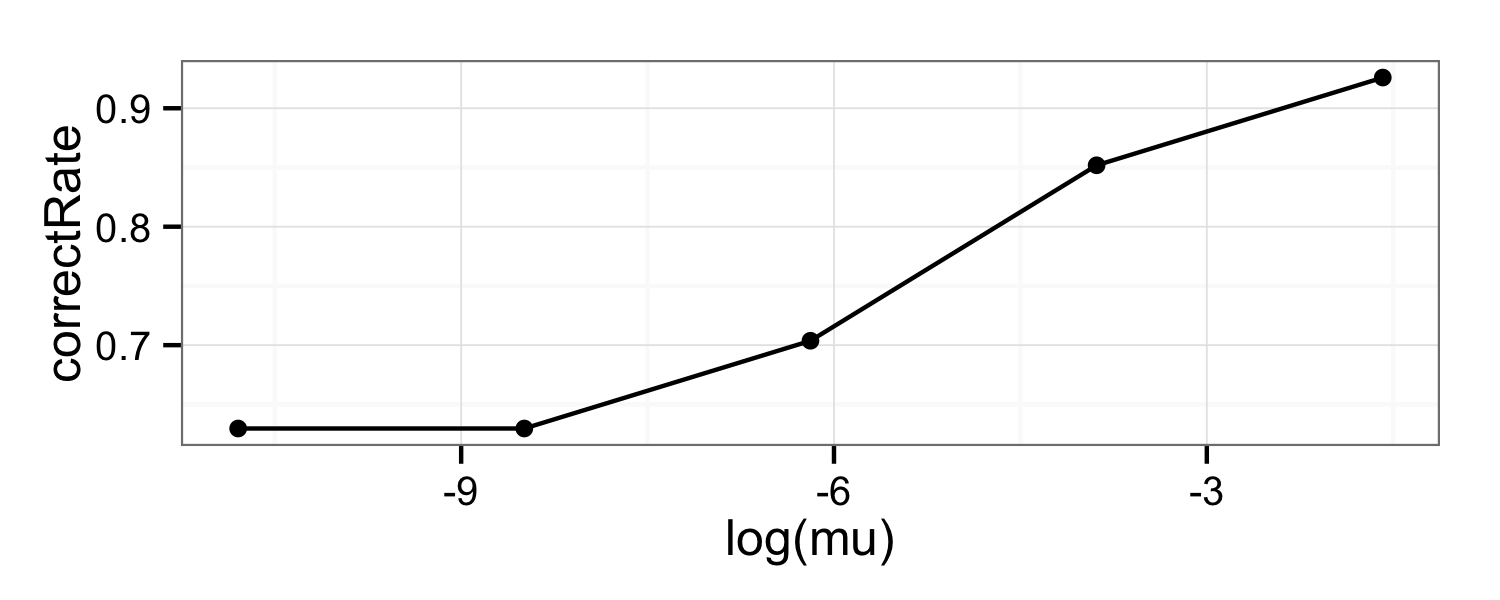
\includegraphics[width=5in]{4c_correctRate.png}
	%\caption{}
	%\label{fig:figName}
\end{figure}

\textbf{False Negative Rate:}
\begin{code}
        mu1 mu2 mu3 mu4    mu5
testSet   0   0   0   0 0.0625
\end{code}

\begin{figure}[H]
	\centering
	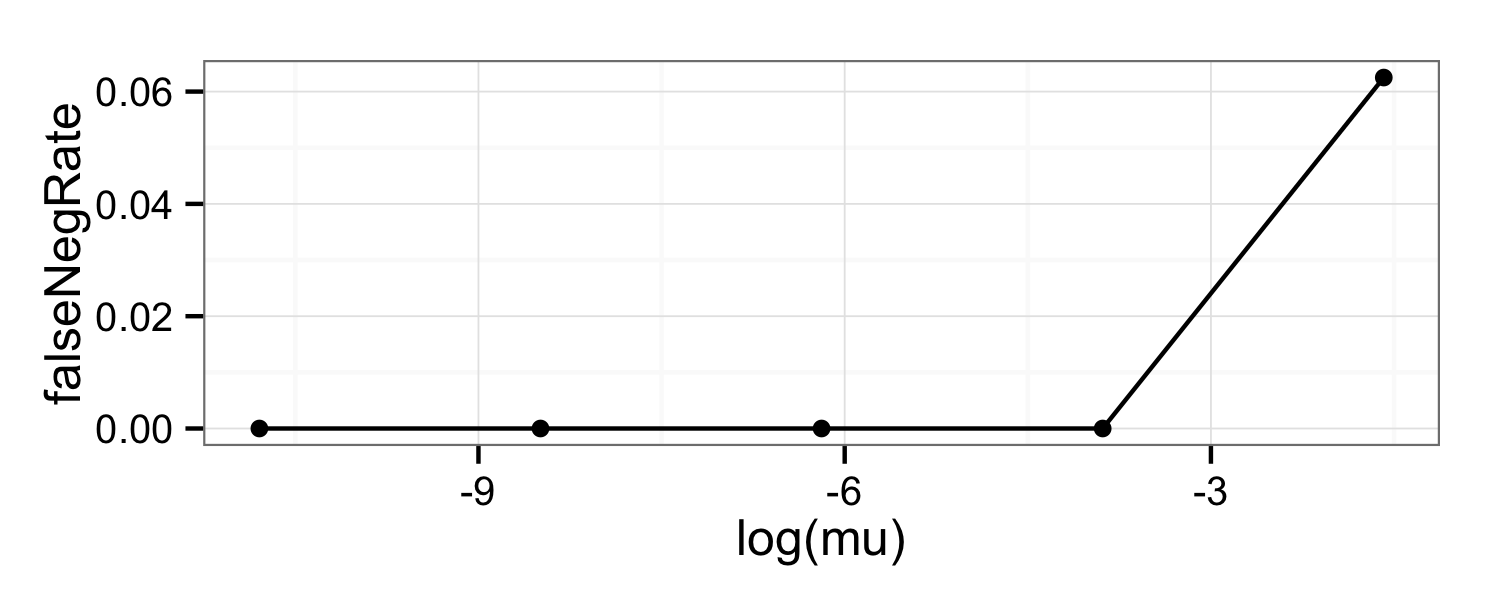
\includegraphics[width=5in]{4c_falseNegRate.png}
	%\caption{}
	%\label{fig:figName}
\end{figure}

\textbf{False Positive Rate:}
\begin{code}
              mu1       mu2       mu3       mu4        mu5
testSet 0.9090909 0.9090909 0.7272727 0.3636364 0.09090909
\end{code}

\begin{figure}[H]
	\centering
	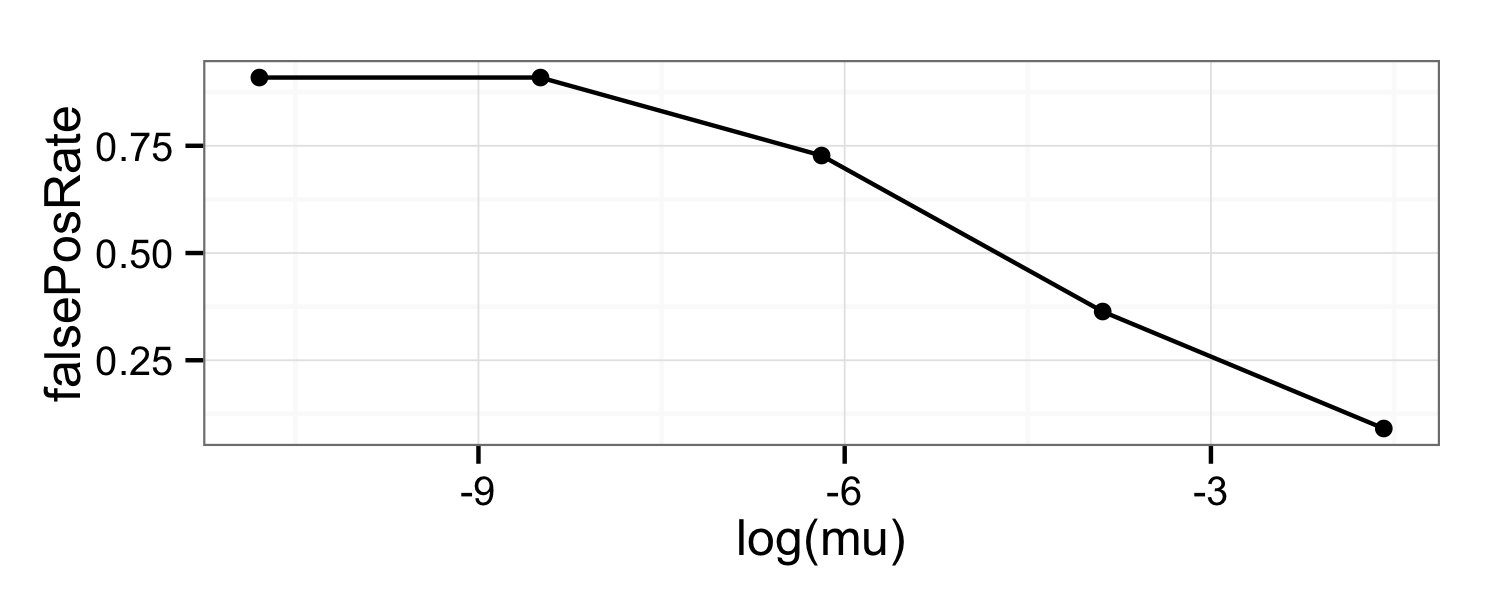
\includegraphics[width=5in]{4c_falsePosRate.png}
	%\caption{}
	%\label{fig:figName}
\end{figure}

Using validation set cross-validation, it still appears as though \texttt{mu5} $=\frac{1000}{\left|D\right|}\approx0.205$ is the optimal choice for $\mu$. At this value we maximize the accuracy and minimize the false positive rate, with only a minimal increase in the false negative rate.
\smallskip

The next-best choice would be \texttt{mu4} $=\frac{100}{\left|D\right|}\approx0.0205$, since at this value we still have a 0\% false negative rate. As we shift from \texttt{mu4} to \texttt{mu5}, however, the large drop in the false positive rate more than compensates for the small increase in the false negative rate, again, making \texttt{mu5} the optimal value.







\part For $\mu=$ \texttt{mu5}, the overall correct rate was more or less accurate, with the cross-validation estimate only 9.28\% lower than the value generated on the full testing set. The false negative and false positive rates show very high percent error --— this is only because both metrics were 0 in the cross-validation estimates and non-zero in the full testing test, making the `percent error' metric somewhat misleading here.
\smallskip

Both the false negative and false positive rates were 0 in the cross-validation estimates, so with non-zero rates generated from the full testing set, the percent error appears to be unreasonably high.
\smallskip

To minimize the differences between the cross-validation rate estimates and the rates on the training set, we could increase the number of folds used in the cross-validation method. This would provide a more accurate estimate for the rate estimates.

\begin{code}
    correctRate falseNegRate falsePosRate
mu1   0.3341176         -Inf   -0.1059259
mu2   0.1435294         -Inf    0.3340741
mu3   0.0800000         -Inf    0.1324074
mu4  -0.1078261         -Inf   -0.1425926
mu5  -0.0928000    -14.81481   -4.3185185
\end{code}








\end{parts}


\end{questions}

%\listoftodos

\end{document}